\section{Hauptsätze der Thermodynamik}

\subsection{Thermodynamische Systeme und ihr Gleichgewicht}

\paragraph{Zustandsvariablen}
Grössen die bestimmbar sind. Bsp: V,p,T

\paragraph{Thermodynamisches System}
Wir bezeichnen mit $S$ ein thermodynamisches System. Eine Abfolge von
Zuständen eines Systems wird mit $\geschwungeneklammer{\sigma_i}_{i=1,\dots,n}$
bezeichnet.

\subsection{Grundbegriffe: System, Prozesse, Zustände, Arbeit}

\subsubsection{Systeme}
Wir nennen die Menge von Systemen $\S$. Jedes System $S \in \S$ ist
aufgebaut aus atomischen (thermodynamischen) Systemen, welche selbts eine
nicht-leere Untermenge $\A \subset \S$ bilden. Atomische Systeme sind in
einem thermodynamischen Sinne unteilbar.

\begin{definition}[Zusammensetzen von Systemen]
    Für eine endliche Anzahl thermodynamischer Systeme $S_1,\dots,S_n \in \S$
    ist das System $S$, welche aus diesen zusammengesetzt ist, definiert
    durch
    \begin{align*}
        \text{Atom}(S) := \text{Atom}(S_1) \cup \dotsb \cup \text{Atom}(S_n)
    \end{align*}
    und wir schreiben $S = S_1 \vee \dotsb \vee S_n$.
\end{definition}

\begin{definition}[Schnitt und disjunkte Systeme]
    Für zwei Systeme $S_1,S_2 \in \S$ ist ihr Schnitt $S_1 \wedge S_2$
    definiert durch
    \begin{align*}
        \text{Atom}(S_1 \wedge S_2) := \text{Atom}(S_1) \cap \text{Atom}(S_2)
    \end{align*}
    Wenn die Schnittmenge $\text{Atom}(S_1) \cap \text{Atom}(S_2)$ leer ist, schreiben
    wir $S_1 \wedge S_2 = \emptyset$ und nennen die Systeme disjunkt.
\end{definition}

\begin{definition}[Untersysteme]
    Für ein System $S \in \S$ ist die Menge seiner Untersysteme definiert durch
    \begin{align*}
        \text{Sub}(S) := \geschwungeneklammer{S' \in \S \ | \ S' \vee S = S}
    \end{align*}
    Für jedes echte Untersystem $S' \in \text{Sub}(S)$, $S' \neq S$, gibt es
    ein eindeutiges disjunktes Komplement $S'' \in \S$, so dass $S' \vee S'' = S$.
\end{definition}


\subsubsection{Prozesse}
Es gibt eine nicht-leere Menge $\P$ von (thermodynamischen) Prozessen.
Jeder Prozess definiert den Anfangs- und Endzustand auf einem atomischen
System $A \in \A$, auf dem er wirkt. Für jedes $A \in \A$ gibt es Funktionen
$\floor{.}_A : \P \rightarrow \Sigma_A$ und $\ceil{.}_A : \P \rightarrow
\Sigma_A$ die einen thermodynamischen Prozess auf den Anfangs- und Endzustand
auf dem System $A$ abbildet und wir sagen, dass das System $A$ in $p$
involviert ist (auch: $p$ wirkt auf $A$). Der Raum $\Sigma_A$ heisst
Zustandsraum von $A$. Für $A_1 \neq A_2$ gilt $\Sigma_{A_1} \cap \Sigma_{A_2}
= \emptyset$. Wir fordern, dass $\forall \ p \in \P$ die Funktionen
$\floor{p}_A$ und $\ceil{p}_A$ für mindestens eines und höchstens endlich
viele $A \in \A$ definiert sind.

\begin{definition}[Zustände allgemeiner Systeme]
    Sei $S = A_1 \vee \dotsb \vee A_n$. Für einen thermodynamischen
    Prozess $p \in \P$ ist der Anfangszustand auf $S$ definiert durch
    \begin{align*}
        \floor{.}_S : \P &\rightarrow \Sigma_S
        \\
        p &\mapsto \floor{p}_S := \klammer{\floor{p}_{A_1},\dots,\floor{p}_{A_n}}
    \end{align*}
    und analog für den Endzustand mittels $\ceil{.}$. Für diskunkte Systeme
    $S_1 , S_2 \in \S$ mit Zuständen $\sigma_1 \in \Sigma_{S_1}$ und $\sigma_2
    \in \Sigma_{S_2}$ verwenden wir die Schreibweise $(\sigma_1 , \sigma_2) =:
    \sigma_1 \vee \sigma_2 = \sigma_2 \vee \sigma_1 \in \Sigma_{S_1} \vee \Sigma_{S_2}$.
\end{definition}

\begin{definition}[Zustandsgrösse]
    Eine Zustandsgrösse eines Systems $S$ (auch Zustandsvariable oder
    Zusatndsfunktion) ist eine Funktion von $\Sigma_S$ in einen Zielraum
    $\mathcal{Z}$, $Z: \Sigma_S \Rightarrow \mathcal{Z}$. Der Zielraum ist
    typischerweise $\mathcal{Z} = \R^n$, meistens sogar $n=1$. Wir schreiben
    $\Delta Z(p) := Z(\ceil{p}_S) - Z(\floor{p}_S)$ für die Änderung einer
    Zustandsgrösse unter einem Prozess $p \in \P$.
\end{definition}

\paragraph{Verknüpfung von Prozessen}
Die Konkatenierung (Hintereinanderausführung) der Prozesse $p,p' \in \P$
zu $p' \circ p$ ist immer mödlich, sobald $\forall A \in \A$ entweder die
Gleichung $\ceil{p}_A = \floor{p'}_A$ gilt, oder mindestens eine der
Seiten undefiniert ist. Ausserdem soll $\circ$ kommutativ sein, für
Prozesse, deren Zustandsänderungen auf disjunkten Untermengen von $\A$
definiert sind. Die Menge der Prozesse $\P$ soll abgeschlossen sein unter
$\circ$. Auf einem beliebigen atomischen System $A \in \A$ gilt:
\begin{align*}
    \floor{p' \circ p}_A = \begin{cases}
        \floor{p}_A \hspace{10pt} &\text{falls } \floor{p}_A \text{ def.}
        \\
        \floor{p'}_A \hspace{10pt} &\text{falls } \floor{p}_A \text{ undef. aber } \floor{p'}_A \text{ def.}
        \\
        \text{undef.} \hspace{10pt} &\text{falls beide } \floor{p}_A \text{ und } \floor{p'}_A \text{ undef.}
    \end{cases}
\end{align*}
sowie Analoges für den Endzustand. Falls $p$ und $p'$ auf disjunkten Systemen
agieren, schreiben wir $p \vee p'$ anstatt $p \circ p' = p' \circ p$.


\paragraph{Arbeitsfunktion}
Für jedes atomisches System $A \in \A$ gibt es eine Arbeitsfunktion
$W_A : \P \rightarrow \R$, welche einem beliebigen Prozess die Arbeit zuordnet,
die während dem Prozess in $A$ investiert wurde. Falls $A$ nicht in $p$
involviert ist, soll $W_A (p) = 0$ gelten. Weiter gilt für $p,p' \in \P$
so dass $p' \circ p$ wohldefiniert ist:
\begin{align*}
    W_A (p' \circ p) = W_A (p) + W_A (p') \ \ \forall A \in \A
\end{align*}
\underline{Konvention}: $W_A$ ist positiv, falls Arbeit aufgewendet werden
muss, also in das System investiert wird. Wenn das System selbst Arbeit
leistet, ist $W_A$ demnach negativ.

\begin{definition}[Arbeitskosten für allgemeine Systeme]
    Für ein beliebiges System $S \in \S$ definieren wir die Arbeitsfunktion
    $W_S : \P \rightarrow \R$ als die Summe der Arbeitsfunktionen der
    Atomischen Untersysteme:
    \begin{align*}
        W_S := \sum_{A \in \text{Atom}(S)} W_A
    \end{align*}
    Für $S_1,S_2 \in \S$ mit $S_1 \wedge S_2 = \emptyset$ und $\forall \ 
    p \in \P$ gilt:
    \begin{align*}
        W_{S_1 \vee S_2} (p) = W_{S_1} (p) + W_{S_2} (p)
    \end{align*}
\end{definition}

\begin{definition}[Identitätsprozess]
    Ein Identitätsprozess soll immer, also für jedes beliebige System in
    jedem beliebigen Anfangszustand, möglich sein. Es ist der Prozess, bei
    dem wir einfach nichts tun. Für so einen Prozess $\id_S^\sigma$ auf $S$
    im Zustand $\sigma$ gilt dann $\floor{\id_S^\sigma}_S = \sigma =
    \ceil{\id_S^\sigma}_S$. Die Arbeitskosten sind Null.
\end{definition}


\subsection{Arbeitsprozesse und der 1. Hauptsatz}

\begin{definition}[Arbeitsprozesse auf $S$]
    Für ein System $S \in \S$ ist $\P_S$ die Menge aller Prozesse, die
    genau auf $S$ wirkt. Wir nennen diese Arbeitsprozesse auf $S$.
    \begin{align*}
        \P_S := \geschwungeneklammer{p \in \P \ | \ \floor{p}_{S'} \text{ ist def. genau für $S' \in \text{Sub}(S)$}}
    \end{align*}
    Arbeitsprozesse auf $S$ sind also Prozesse, für welche $S$ das "grösste"
    System ist, auf dem sie wirken.
\end{definition}

\begin{definition}[Zyklische und Identitätsprozesse]
    Ein thermodynamischer Prozess $p \in \P$ heisst zyklisch auf $S \in \S$,
    falls $\floor{p}_S = \ceil{p}_S$. Er heisst Identitätsprozess, wenn er
    ein Arbeitsprozess $p \in \P_S$ auf $S$ ist. Für Identitätsprozesse auf
    $S$, die den Zusatand $\sigma$ invariant lassen, benutzen wir die Notation
    $p = \id_S^\sigma = \id_S$. 
\end{definition}

\begin{definition}[Reversibler Arbeitsprozess]
    Ein Arbeitsprozess $p \in \P_S$ auf einem System $S$ heisst reversibel,
    falls es einen Arbeitsprozess $p^{rev} \in \P_S$ gibt, so dass
    $p^{rev} \circ p$ ein Identitätsprozess ist. Insbesondere ist dann
    $p^{rev} \circ p$ definiert.
\end{definition}

\paragraph{1. Hauptsatz}
Für jedes System $S \in \S$ gilt:
\begin{enumerate}[(i)]
    \item Zu jedem Paar von Zuständen $\sigma_1 , \sigma_2 \in \Sigma_S$
        gibt es einen Arbeitsprozess $p \in \P_S$ auf diesem System, so dass
        $\floor{p}_S = \sigma_1$ und $\ceil{p}_S = \sigma_2$ oder es gibt
        $p' \in \P_S$ so dass $\floor{p'}_S = \sigma_2$ und $\ceil{p'}_S =
        \sigma_1$.
    \item Die Arbeitskosten eines Prozesses $p \in \P_S$ mit Anfangszustand
        $\sigma_1$ und Endzustand $\sigma_2$ hängt nur vom geordneten Paar
        $(\sigma_1,\sigma_2)$ ab und nicht vom Prozess $p$. D.h. falls es
        einen anderen Prozess $p'' \in \P_S$ gibt, welcher die gleichen
        Zustände in der gleichen Richtung ineinander überführt, so gilt
        $W_S (p'') = W_S (p)$.
\end{enumerate}

\begin{bemerkung}
    Es gilt $W_S(\id_S^\sigma) = 0$. Weiter gilt für jeden reversiblen
    Arbeitsprozess $p \in \P_S$ mit Umkehrprozess $p^{rev} \in \P_S$:
    \begin{align*}
        W_S (p^{rev}) = - W_S(p)
    \end{align*}
\end{bemerkung}

\begin{definition}[Innere Energie]
    Die (innere) Energie eines Systems $S$ im Zustand $\sigma \in \Sigma_S$
    ist definiert als
    \begin{align*}
        U_S (\sigma) &:= W_S + U_0
        \hspace{10pt} , \hspace{10pt}
        \text{falls } p \in \P_S \ \sigma_0 \text{ in } \sigma \text{ überführt}
        \\
        U_S (\sigma) &:= - W_S (p') + U_0
        \hspace{10pt} , \hspace{10pt}
        \text{falls } p' \in \P_S \ \sigma \text{ in } \sigma_0 \text{ überführt}
    \end{align*}
    Wobei $\sigma_0 \in \Sigma_S$ ein beliebiger aber fixer Referenzzustand ist
    und $U_0 \in \R$ eine willkürkliche aber fixe Energiekonstante.
\end{definition}


\subsection{Wärme}

\begin{definition}[Wärme]
    Sei $p \in \P$ ein beliebiger Prozess. Dann ist die $S$ zufliessende
    Wärme definiert als
    \begin{align*}
        Q_S (p) := \Delta U_S (p) - W_S (p)
        \hspace{10pt} , \hspace{10pt}
        \Delta U_S (p) := \sum_{\stackrel{A \in \text{Atom}(S)}{A \text{ inv. in } p}} \Delta U_A (p)
    \end{align*}
    Wärme ist also die Energie, die zwischen Systemen ausgetauscht wird
    und dadurch die innere Energie der betroffenen Systeme verändert, welche
    nicht Arbeit ist.
\end{definition}

\paragraph{Notation} $W_S := W_S(p)$ und $Q_S = Q_S(p)$

\begin{definition}[Quasistatischer Prozess]
    Ein quasistatischer Arbeitsprozess auf einem System $S \in \S$ ist eine
    zweiparametrige Familie von Arbeitsprozessen
    $\geschwungeneklammer{p(\lambda,\lambda')}_{\lambda,\lambda'} \subset
    \P_S$ mit $\lambda,\lambda' \in [0,1]$ und $\lambda \leq \lambda'$
    und den Eigenschaften:
    \begin{enumerate}[(i)]
        \item Für $\lambda \leq \lambda' \leq \lambda'' \in [0,1]$ gilt
            $p(\lambda',\lambda'') \circ p(\lambda,\lambda') = p(\lambda,\lambda'')$
            $\Rightarrow \ceil{p(\lambda,\lambda')}_S = \floor{p(\lambda',\lambda'')}_S
            \ \forall \lambda \leq \lambda' \leq \lambda''$.
        \item Der Pfad $\lambda \mapsto \sigma_{\lambda} := \floor{p(\lambda,\lambda')}_S$
            ist stetig.
        \item Für alle $A \in \text{Atom}(S)$ ist $W_A(p(\lambda,\lambda'))$ stetig
            in $\lambda$ und $\lambda'$ auf ihrem Definitionsbereich.
    \end{enumerate}
    Quasistatische Prozesse sind solche, welche eine kontinuierliche
    Aufteilung in Teilprozesse erlauben.
\end{definition}

\begin{definition}[Differentielle Arbeit und Wärme]
    Sei $\geschwungeneklammer{p(\lambda,\lambda')}_{\lambda,\lambda'}$
    ein quasistatischer Arbeitsprozess auf $S$ mit einem stückweise stetig
    differenzierbaren Pfad $\lambda \mapsto \sigma_\lambda$ in $\Sigma_S$.
    Eine $1$-Form $\delta^{(p)} W_A$ heisst differentielle Arbeit auf $A
    \in \text{Atom}(S)$ falls für alle $\lambda \leq \lambda' \in [0,1]$
    gilt
    \begin{align*}
        W_A (p(\lambda,\lambda')) &=
        \int_{\sigma_\lambda}^{\sigma_{\lambda'}} \delta^{(p)} W_A
        \\
        \delta^{(p)} W_A (\lambda) &=
        \frac{d}{d \lambda'} \Big|_{\lambda' = \lambda} W_A (p(\lambda',\lambda)) \ d \lambda
    \end{align*}
    Die differentielle Wärme auf $A \in$ Atom$(S)$ ist die $1$-Form gegeben durch
    \begin{align*}
        \delta^{(p)} Q_A := d U_A - \delta^{(p)} W_A
    \end{align*}
\end{definition}

\begin{bemerkung}
    Das Superscript $(p)$ steht für den quasistatischen Prozess. Die
    differentielle Arbeit $\delta^{(p)} W_{S'}$ und die differentielle
    Wärme $\delta^{(p)} Q_{S'}$ sind keine exakten $1$-Formen, wie $dU$ es
    ist. Differentielle Arbeit und Wärme sind pfad- und prozessabhängig.
    Die Arbeit $W_S$ is also keine Zustandsgrösse. Die Aussage, dass $dU$
    ein exaktes Differential ist, heisst dann, dass das Integral unabhängig
    vom Pfad ist, über den integriert wird. Insbesondere gilt dann für
    einen zyklischen Prozess $\oint dU = 0$ und $W_S = - Q_S$.
\end{bemerkung}

\begin{bemerkung}
    Arbeitsprozesse haben die Eigenschaft, dass keine Wärme dem System zugeführt
    oder vom System abgeführt wird.
\end{bemerkung}

\begin{definition}[Adiabatische Prozesse]
    Ein quasistatischer Prozess $p \in \P_S$, der unter anderem auf $S$ wirkt,
    heisst adiabatische auf $S$, falls $\delta Q_S = 0$.
\end{definition}

\begin{bemerkung}
    Ein quasistatischer Arbeitsprozess $p \in \P_S$ auf $S$ ist adiabatisch, da
    für solche immer $dU_S = \delta W_S$ per Definition von $U_S$ gilt. Desshalb
    $\delta Q_S = 0$.
\end{bemerkung}


\subsection{Der 2. Hauptsatz}

\paragraph{2. Hauptsatz}
"Kein Prozess ist möglich, dessen einziges Resultat darin besteht, dass einem
System Wärme entzogen und Arbeit geleistet wird."

\begin{definition}[Äquivalente Systeme]
    Zwei Systeme $S_1$ und $S_2$ heissen äquivalent, wenn ihre thermodynamischen
    Eigenschaften identisch sind. Wir schreiben dann $S_1 \cong S_2$.
\end{definition}

\begin{definition}[Thermisches Reservoir]
    Ein System $R \in \S$ heisst thermisches Reservoir (auch Wärmereservoir
    oder einfach Reservoir) falls es folgende Annahmen erfüllt:
    \begin{enumerate}[(i)]
        \item Die Zustandsfunktion $U_R : \Sigma_R \rightarrow \R$ ist injektiv.
            D.h. die innere Energie bestimmt den Zustand von $R$ eindeutig.
        \item Für alle Prozesse $p \in \P$ gilt $W_R(p) \geq 0$. Aus einem
            Reservoir kann also nie Arbeit extrahiert werden.
        \item Zwei Kopien $R \cong R'$ eines Reservoirs können immer durch ein
            weiteres Reservoir $R''$ mit $R \cong R''$ und $R' \cong R''$ ersetzt
            werden. D.h. ein Arbeitsprozess $p \in \P_{R \vee R' \vee S}$ auf $R$,
            $R'$ und einem System $S \in \S$ kann immer zu einem Arbeitsprozess
            $\overline{p} \in \P_{R'' \vee R \vee R' \vee S}$ erweitert werden, so
            dass die Wärme nur noch aus $R''$ kommt. Formal fordern wir für die
            Erweiterung $\overline{p}$: $R$ wie $R'$ sind zyklisch unter $\overline{p}$
            mit $W_{R \vee R'} (\overline{p}) = 0$, $W_{R''} (\overline{p}) = W_{R \vee R'} (p)$,
            $W_{S'} (\overline{p}) = W_{S'} (p)$ für alle anderen Systeme, sowie
            $\floor{\overline{p}}_S = \floor{p}_S$ und $\ceil{\overline{p}}_S =
            \ceil{p}_S$.
    \end{enumerate}
    Manchmal wird in der zweiten Aussage auch gefordert, dass $W_R(p) = 0$ und
    die dritte Aussage kann man umformulieren zu:
    \begin{enumerate}[]
        \item $\forall p \in \P \ \forall \Delta U \in \R \ \exists p'$ s.d.
            $p'$ identisch ist zu $p$ ausser $\floor{p'} = \floor{p} + \Delta U$
            und $\ceil{p'} = \ceil{p} + \Delta U$.
    \end{enumerate}
\end{definition}

\begin{bemerkung}
    Für $\sigma_1,\sigma_2 \in \Sigma_R$ mit $U_R (\sigma_2) > U_R (\sigma_1)$
    existiert immer ein Arbeitsprozess $p \in \P_R$ auf $R$ mit $W_R(p) =
    U_R (\sigma_2) - U_R (\sigma_1) \geq 0$ und $\floor{p}_R = \sigma_1$,
    $\ceil{p}_R = \sigma_2$.
\end{bemerkung}

\paragraph{2. Hauptsatz}
Wir können den 2. Hauptsatz umformulieren zu:
\begin{enumerate}[]
    \item Sei $S \in \S$ ein beliebiges System und $R \in \S$ ein Reservoir.
        Dann gilt $\forall p \in \P_{S \vee R}$, welche zyklisch sind auf $S$,
        dass $W_S(p) \geq 0$.
\end{enumerate}

\begin{bemerkung}
    Für einen reversiblen Prozess $p \in \P_{S \vee R_1 \vee \dotsb \vee R_n}$
    auf einem beliebigen System $S \in \S$ und einer Kollektion von Reservoirs
    $R_1,\dots,R_n$ dass für jeden beliebigen Umkehrprozess $p^{rev} \in
    \P_{S \vee R_1 \vee \dotsb \vee R_n}$ gilt:
    \begin{align*}
        W_S(p^{rev}) &= - W_S(p)
        \\
        W_{R_i} (p^{rev}) &= - W_{R_i}(p) \ \ \forall i = 1,\dots,n
        \\
        Q_{R_i} (p^{rev}) &= - Q_{R_i}(p) \ \ \forall i = 1,\dots,n
    \end{align*}
\end{bemerkung}


\subsection{Das Carnot Theorem}

\begin{minipage}{0.09\textwidth}
    \begin{center}
        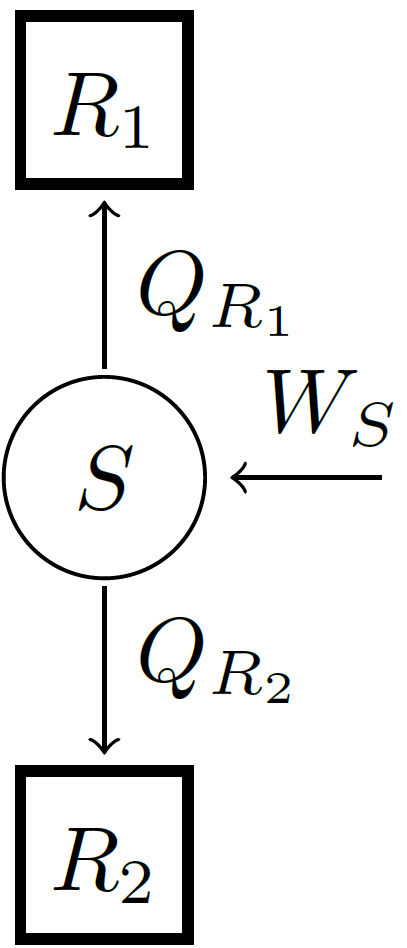
\includegraphics[width=0.9\textwidth]{Bilder/Carnot_Thm.png}
    \end{center}
\end{minipage} \hspace{2pt}
\begin{minipage}{0.39\textwidth}
    Ein System $S \in \S$, von nun an als "Maschine" bezeichnet, operiert
    zyklisch zwischen zwei Reservoirs $R_1,R_2 \in \S$, welche nicht
    Kopien voneinander sein müssen. Auf $S \vee R_1 \vee R_2$ findet also
    ein Arbeitsprozess $p \in \P_{S \vee R_1 \vee R_2}$ statt, der zyklisch
    auf $S$ ist. Ausserdem wird nur direkt in $S$ Arbeit investiert respektive
    von $S$ extrahiert, nämlich $W_S := W_S (p)$. Für die Reservoirs soll
    gelten $W_{R_1}(p) = W_{R_2}(p) = 0$. Wir betrachten die Wärmeflüsse zu
    den Reservoirs, $Q_{R_1} := Q_{R_1}(p)$ und $Q_{R_2} := Q_{R_2}(p)$, wobei
    wir annehmen, dass diese nicht null sind.
\end{minipage}

\begin{bemerkung}
    Wegen dem 1. Hauptsatz und der Zyklizität des Prozesses auf $S$ folgt
    $W_S = - Q_S$. Weiter gilt wegen $W_{R_1}(p) = W_{R_2}(p) = 0$:
    \begin{align*}
        W_S = W_{S \vee R_1 \vee R_2} = \Delta U_{S \vee R_1 \vee R_2}
    = \Delta U_{R_1} + \Delta U_{R_2} = Q_{R_1} + Q_{R_2}
    \end{align*}
\end{bemerkung}

\begin{lemma}
    Wir betrachten eine Situation wie oben beschrieben. Insbesondere sind
    nicht beide Wärmeflüsse $Q_{R_1}$ und $Q_{R_2}$ gleichzeitig null. Für
    alle solchen $p \in \P_{S \vee R_1 \vee R_2}$ gelten folgende Aussagen:
    \begin{enumerate}[(i)]
        \item $Q_{R_1} \leq 0$ und $Q_{R_2} \leq 0$ können nicht gleichzeitig gelten.
        \item Falls $p$ zusätzlich reversibel ist, so gilt $\frac{Q_{R_1}}{Q_{R_2}} < 0$.
    \end{enumerate}
\end{lemma}

\paragraph{Carnots Theorem}
Betrachte eine zyklische Maschine $S \in \S$, die unter dem reversiblen
Prozess $p \in \P_{S \vee R_1 \vee R_2}$ zwischen zwei Reservoirs $R_1,R_2
\in \S$ operiert. Die Einschränkungen seien wie oben beschrieben. Sei $S' \in
\S$ eine weitere solche Maschine, die unter $p' \in \P_{S' \vee R_1 \vee R_2}$
zwischen identischen Reservoirs operiert, jedoch nicht unbedingt reversibel.
Es ist immer mindestens ein Wärmefluss positiv nach obigem Lemma. Wir wählen
o.B.d.A. $Q_{R_2}(p') > 0$. Wir wählen die Richtung des reversiblen Prozesses
so, dass er in die gleiche Richtung arbeitet, das heisst $Q_{R_2} > 0$. Dann
gilt:
\begin{enumerate}[(i)]
    \item Die Verhältnisse der Wärmeflüsse erfüllen:
        \begin{align*}
            - \frac{Q_{R_1}(p')}{Q_{R_2}(p')} \leq - \frac{Q_{R_1}(p)}{Q_{R_2}(p)}
            := \tau(R_1,R_2) > 0
        \end{align*}
        mit Gleichheit falls $p'$ reversibel ist.
    \item Das Verhältnis $- \frac{Q_{R_1}(p)}{Q_{R_2}(p)}$ für die reversible
        Maschine hängt nur von den beiden Reservoirs $R_1$ und $R_2$ ab und
        nicht von der verwendeten zyklischen Maschine $S$ oder vom genauen
        Prozess $p$. Es ist in diesem Sinne universell.
\end{enumerate}
Eine äquivalente Beschreibung ist:
\begin{enumerate}[]
    \item $\exists \tau(R_1,R_2) \rightarrow \R$ s.d. $\forall S$ und
        $\forall p \in \P_{S \vee R_1 \vee R_2}$ zyklisch auf $S$ mit
        $Q_{R_2}(p) > 0$ gilt $- \frac{Q_{R_1}(p)}{Q_{R_2}(p)} \leq
        \tau(R_1,R_2) > 0$ mit gleichheit falls $p$ reversibel ist.
\end{enumerate}

\subsection{Absolute Temperatur}

\begin{definition}[$\tau$]
    Für das Verhältnis der mit einer nicht-trivialen reversiblen zyklischen
    Maschine ausgetauschten Wärmeflüsse mit zwei Reservoirs $R_1$ und $R_2$,
    definieren wir die Funktion
    \begin{align*}
        \tau(R_1,R_2) := - \frac{Q_{R_1}}{Q_{R_2}}
    \end{align*}
    Dabei sei $Q_{R_2} > 0$ der positive Wärmefluss. Es gilt $\tau > 0$.
\end{definition}

\begin{lemma}
    Seien $R_1,R_2,R_2$ drei beliebige verschiedene Reservoirs. Dann gilt:
    \begin{enumerate}[(i)]
        \item $\tau(R_1,R_2) \tau(R_2,R_3) = \tau(R_1,R_3)$
        \item $\tau(R,R) = 1$
        \item $\tau(R_1,R_2) = \klammer{\tau(R_2,R_1)}^{-1}$
    \end{enumerate}
\end{lemma}

\begin{definition}[Absolute Temperatur]
    Wir wählen ein beliebiges aber fixes "Referenz-Reservior" $R_{ref} \in
    \mathcal{R}$ sowie eine beliebige fixe positive Konstante $T_{ref} \in
    \R_{>0}$. Die absolute Temperatur eines Reservoirs $R$ ist definiert als
    \begin{align*}
        T := \tau(R,R_{ref}) T_{ref}
    \end{align*}
\end{definition}

\begin{lemma}
    Allgemein: $T_2 = \tau(R_2,R_1)T_1$ und somit
    $\tau(R_2,R_1) = \frac{T_2}{T_1}$.
\end{lemma}

\begin{definition}[Wärmekraftmaschine und Wärmepumpe]
    Wir nennen eine zyklische Maschine $S$, die zwischen zwei Reservoirs
    arbeitet eine Wärmekraftmaschine, falls sie Arbeit produziert, falls also
    Arbeit extrahiert werden kann. In unserer Konvention heisst das $W_S < 0$. Falls das
    umgekehrte der Fall ist, $W_S > 0$, wird Arbeit benutzt, um die Wärme vom
    kälteren ins heissere Wärmebad zu transportieren. In diesem Fall nennen
    wir die Maschine eine Wärmepumpe.
\end{definition}

\begin{definition}[Wirkungsgrad $\eta$]
    Die Effizienz einer nicht-trivialen reversiblen zyklischen Wärmekraftmaschine
    $S$, definiert als $\eta := \frac{\abs{W_S}}{\abs{Q_{R_1}}}$, wobei $Q_{R_1}$
    der negativen Wärmefluss ist, kann geschrieben werden als $1 - \frac{T_2}{T_1}$,
    wobei $T_1 > T_2$ die Temperaturen der beiden Reservoirs sind, die die
    Maschine nutzt um Arbeit zu produzieren. Eine beliebige andere
    Wärmekraftmaschine (nicht unbedingt reversible) kann höchstens diese
    Effizienz erreichen. Die maximale Effizienz $\eta_C := 1 - \frac{T_2}{T_1}$,
    auch Carnot Effizienz genannt, hängt also nur von den Temperaturen der
    involvierten Reservoirs ab.
\end{definition}

\begin{definition}[Leistungszahl]
    Für die Wärmepumpen kann man eine analoge Aussage machen. Die Leistungszahl
    (auch Heizzahl oder Coefficient of Performance COP) einer Wärmepumpe ist
    definiert als das Verhältnis der von der Maschine abgegebene Wärme zu
    investierter Arbeit. Die Leistungszahl ist von oben beschränkt:
    \begin{align*}
        \text{COP} := \frac{Q_{R_2}}{W_S} \leq \frac{1}{1 - \frac{T_1}{T_2}}
    \end{align*}
\end{definition}

\paragraph{0. Hauptsatz}
Zwei Reservoirs $R_1$ und $R_2$ sind im Gleichgewicht, wenn $\tau(R_1,R_2)
= 1$, also wenn sie die gleiche Temperatur haben. Wir schreiben $R_1 \sim R_2$.
Insbesondere identische Reservoirs $R \cong R'$ erfüllen $R \sim R'$. Der
0. Hauptsatz besagt: Wenn System $A$ und $B$ im thermischen Gleichgewicht
sind und Systeme $B$ und $C$ ebenfalls, dann sind auch $A$ und $C$ im
thermischen Gleichgewicht.

\begin{definition}[Temperatur eines Wärmeflusses]
    Sei $S = S_1 \vee S_2 \in \S$ ein disjunkt bipartites System, auf welchem
    ein Arbeitsprozess $p \in \P_S$ ausgeführt wird. Wir schreiben $W_i :=
    W_{S_i}(p)$ und $Q := Q_{S_2}(p)$. Für $Q \neq 0$ sagen wir, die Wärme
    zwischen $S_1$ und $S_2$ fliesst bei Temperatur $T$, falls zwei Reservoirs
    $R_1$ und $R_2$, beide bei Temperatur $T$, zusammen mit zwei Prozessen
    $p_1 \in \P_{S_1 \vee R_1}$ und $p_2 \in \P_{S_2 \vee R_2}$ existieren,
    so dass $W_{S'}(p_i) = W_{S'}(p)$ für alle Systeme $S' \in \S$ welche
    keinen Überlapp mit dem anderen System haben, $S' \wedge S_{i+1} = \emptyset$,
    und die Zustandsänderungen auf den $S_i$ unter $p_i$ beibehalten werden,
    $\floor{p_i}_{S_i} = \floor{p}_{S_i}$ sowie $\ceil{p_i}_{S_i} = \ceil{p}_{S_i}$.
\end{definition}

\begin{lemma}
    Wenn man dem Wärmefluss eine Temperatur zuordnen kann, sind die
    Teilprozesse $p_i \in \P_{S_i \vee R_i}$ reversibel und die Temperatur
    des Wärmeflusses eindeutig.
\end{lemma}


\subsection{Clausius' Theorem und Entropie}

Aus vorherigen Erkentnissen folgt: $- \frac{Q_1}{Q_2} = \frac{T_1}{T_2}
\Leftrightarrow \frac{Q_1}{T_1} + \frac{Q_2}{T_2} = 0$ für reversible
Prozesse. Allgemein folgt:

\paragraph{Clausius' Theorem}
Sei $S \in \S$ ein beliebiges System und $\geschwungeneklammer{R_i}_{i=1}^N$
eine Menge von Reservoirs, so dass $R_i$ die Temperatur $T_i$ hat. Für jedes
$i=1,\dots,N$ sei $p_i \in \P_{S \vee R_i}$ ein Arbeitsprozess auf $S$ und
dem Reservoir $R_i$ mit $W_{R_i}(p_i) = 0$, so dass der Prozess $p := p_N
\circ \dotsb \circ p_1$ definiert ist und insgesamt zyklisch auf $S$. Dann gilt
\begin{align*}
    \sum_i \frac{Q_S (p_i)}{T_i} \leq 0
\end{align*}
mit Gleichheit wenn $p$ reversibel ist.
Für quasistatische Prozesse wie im Clausius Theorem beschrieben gilt:
\begin{align*}
    \oint \frac{\delta Q_s}{T} \leq 0
\end{align*}
wieder mit Gleichheit falls $p$ reversibel ist.

\begin{definition}[Entropie]
    Sei $S \in \S$ ein System und $\sigma_{ref} \in \Sigma_S$ ein beliebiger
    aber fixer Zustand darauf. Sei $S_{ref} \in \R$ eine beliebige reelle
    Konstante. Für einen Zustand $\sigma \in \Sigma_S$ definieren wir die
    Entropie
    \begin{align*}
        S_S (\sigma) := \sum_{i=1}^N \frac{Q_S (p_i)}{T_i} + S_{ref}
    \end{align*}
    wobei die Summe über die reversiblen Teilprozesse $p_i$ wie im Clausius
    Theorem geht, so dass das System $S$ während den $p_i$ die Wärme $Q_S(p_i)$
    bei Temperatur $T_i$ austauscht und $p = p_N \circ \dotsb \circ p_1$ so ist,
    dass $\floor{p}_S = \sigma_{ref}$ und $\ceil{p}_S = \sigma$. Falls die
    beteiligten Prozesse quasistatisch sind, kann man die Definition auch
    schreiben als
    \begin{align*}
        S_S (\sigma) := \int_{\sigma_{ref}}^\sigma \frac{\delta Q_S}{T} + S_{ref}
    \end{align*}
    Wir definieren das exakte Differential $dS = \frac{\delta Q_S}{T}$.
\end{definition}

\begin{theorem}[Entropiesatz]
    In einem adiabatischen Prozess kann die Entropie eines Systemes nicht
    abnehmen, d.h. für einen adiabatischen Prozess $p \in \P$ auf einem
    System $S$ gilt:
    \begin{align*}
        \Delta S_S (p) \geq 0
        \hspace{20pt} \Leftrightarrow \hspace{20pt}
        S_S(\floor{p}_S) \leq S_S(\ceil{p}_S)
    \end{align*}
    und es gilt Gleichheit, falls der Prozess reversibel ist.
\end{theorem}

\begin{bemerkung}
    Mit unserem bisherigen Wissen folgern wir, dass
    \begin{align*}
        dU = T dS - p dV
    \end{align*}
    Während einem Prozess, in dem dass das Volumen $V$ konstant gehalten wird,
    gilt dann
    \begin{align*}
        T = \frac{\partial U}{\partial S} \Big|_V
    \end{align*}
    Da $T$ ausgedrückt werden kann durch Zustandsgrössen, ist $T$ also eine
    Zustandsgrösse und wird Temperatur des Systems genannt.
\end{bemerkung}
